\chapter{EVALUATION, RESULTS AND OUR CONTRIBUTION }\label{our_work}

Yazilacak.

\section{Framework}

One of the key points in our study was to create a model that allows many different models to work together. In order to achieve this, we had to create a framework that is easily accessible by different models and consists of parts that generate standard types of feedback. In this way, we would have obtained a modular structure where it is easy to make changes and incorporate new ideas. General structure of our framework is shown in Figure \ref{fig:framework}.

\begin{figure}[h]
    \centering
    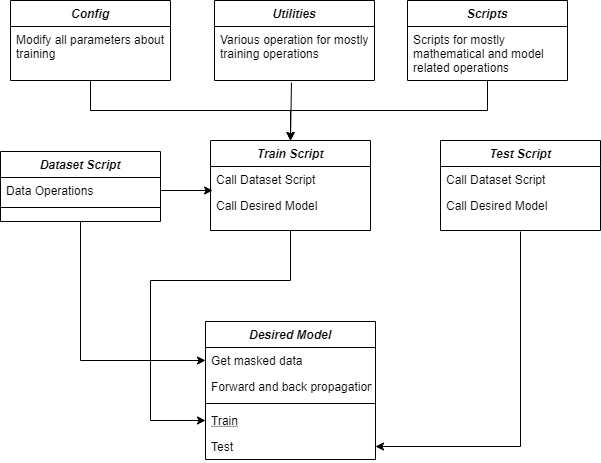
\includegraphics[scale=0.6]{figures/chapter5/framework (1).png}
    \caption{Framework}
    \label{fig:framework}
\end{figure}
In order to provide these, we created scripts that will serve as small building blocks. The most important of these building blocks are the dataset and utilities scripts, which are also actively used by models and can include important features of the models.
\newline
Masked images or transformed images that models use as input are also generated by the dataset script. We created 2 different types of masking. The first masking type we have created is the masking type that creates scattered lines on the picture which we call line masking. With this masking type, we are able to simulate smaller imperfections rather than large missing regions in the picture. Line masking example is shown in Figure \ref{fig:linemasking}.

\begin{figure}[h]
    \centering
    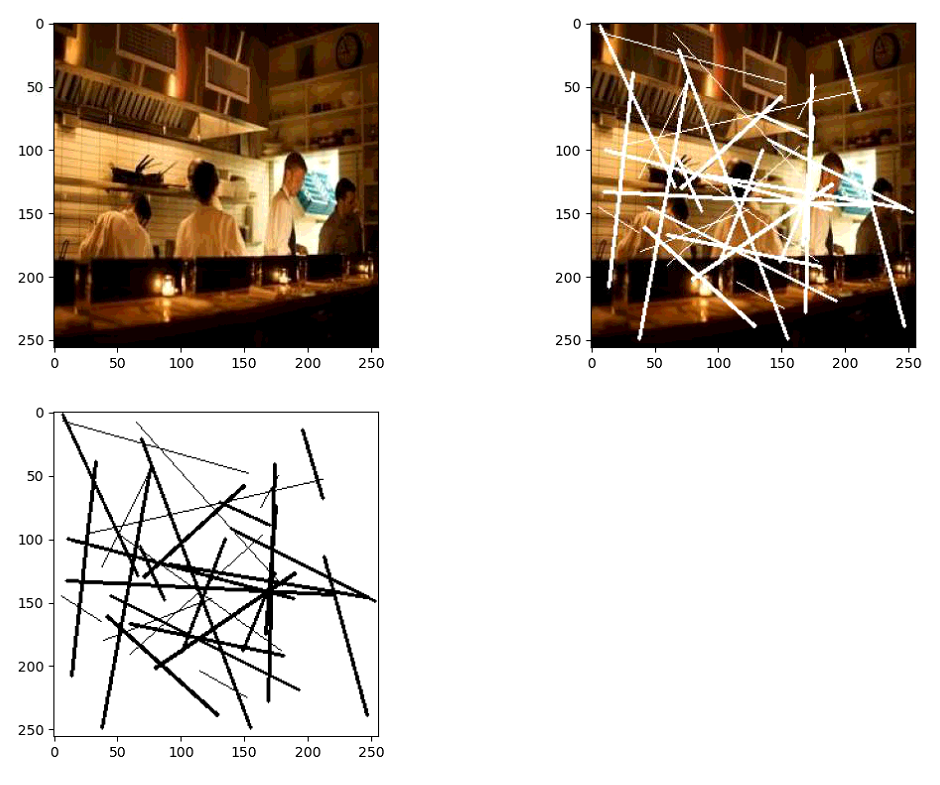
\includegraphics[scale=0.5]{figures/chapter5/linemasking.PNG}
    \caption{Line Masking Example !!DUZELTILECEK}
    \label{fig:linemasking}
\end{figure}

The other masking function we use is a function that masks a region of the given ratio value, starting from a random point on the picture. We preferred to use this masking type more to show that generative models are more successful. Our second masking type is presented in \ref{fig:percentagemasking}.

\begin{figure}[h]
    \centering
    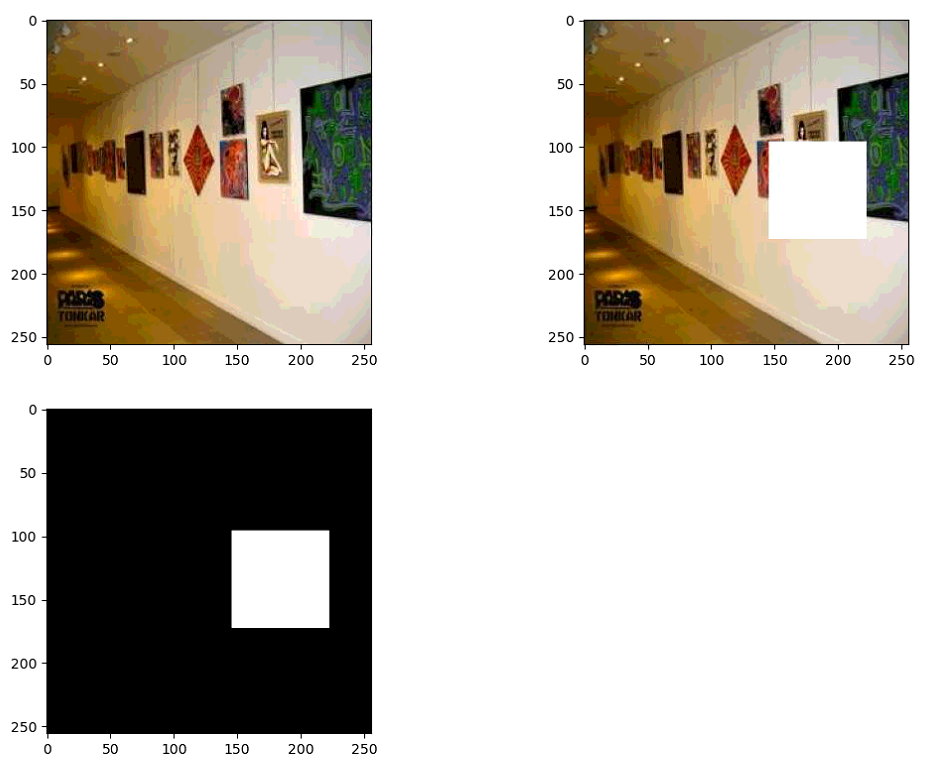
\includegraphics[scale=0.5]{figures/chapter5/percentageMasking.PNG}
    \caption{Percentage Masking Example !!DUZELTILECEK}
    \label{fig:percentagemasking}
\end{figure}

Image inpainting, unfortunately, is not a method whose success can be fully controlled with mathematical methods. However, PSNR and SSIM values will be used throughout the project as a criterion in addition to achieving personal realistic results. An example of image inpainting with one of our mathematical method is shown in Figure \ref{fig:mathmodel}.

\begin{figure}[h]
    \centering
    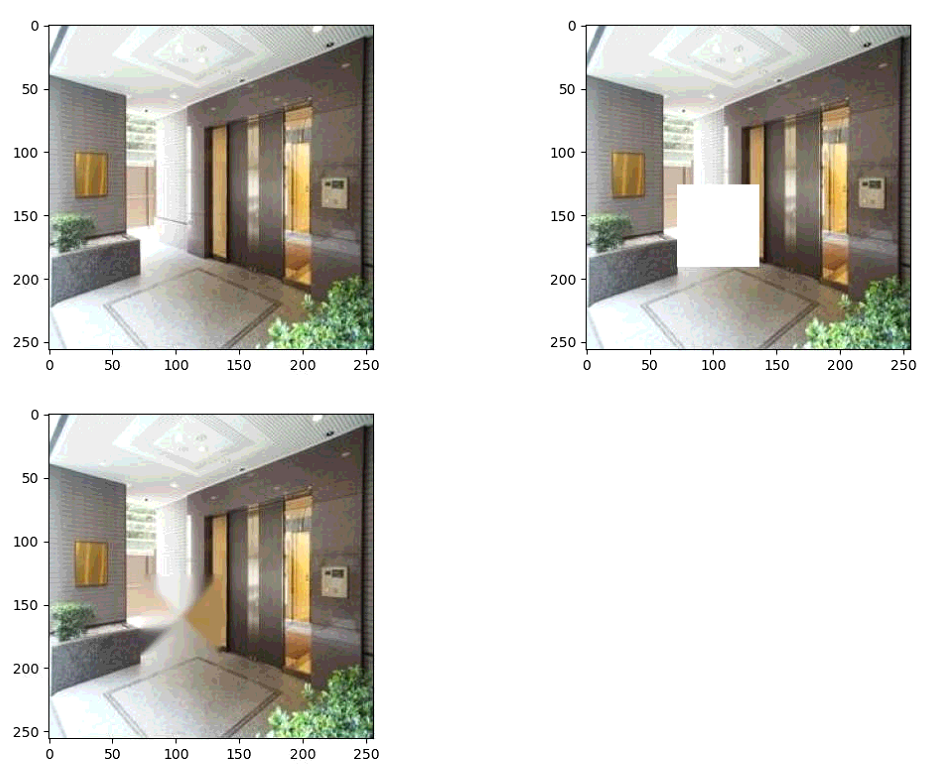
\includegraphics[scale=0.4]{figures/chapter5/testMath.PNG}
    \caption{Mathematical Modedl Example !!DUZELTILECEK}
    \label{fig:mathmodel}
\end{figure}

\section{Our Contribution}

\subsection{Unified Contextual-Edge Model}
During our literature review we studied a model by Yu et al. which is called Free-Form Image Inpainting with Gated Convolution \cite{freeform_inpainting}. In this model, there are 3 main stages as shown in the Figure \ref{fig:freeform}.

\begin{figure}[h]
    \centering
    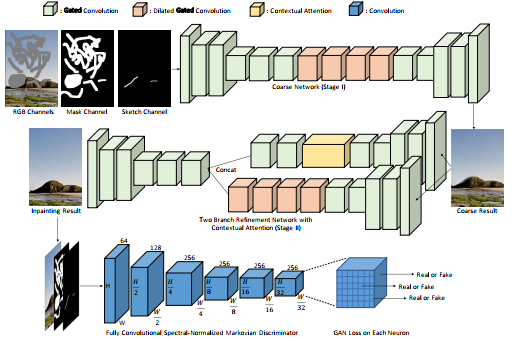
\includegraphics[scale=0.5]{figures/chapter5/Free-form.PNG}
    \caption{Free-form Image Inpainting Example}
    \label{fig:freeform}
\end{figure}

Based on this, we wanted to try EdgeConnect and Generative Contextual Attention models in a cascaded network. Hence, there will be 3 steps in the new model. Which consists of following steps. figure \ref{fig:unifiedIdeda} shows the steps of this model. 


\begin{figure}[h]
    \centering
    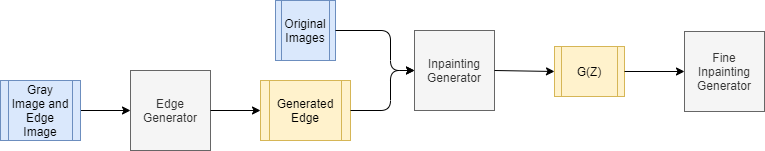
\includegraphics[scale=0.5]{figures/chapter5/Unified.png}
    \caption{Unified Model Structure}
    \label{fig:unifiedIdeda}
\end{figure}

•	Edge information prediction \newline
•	Inpainting operation with edge and RGB image as input \newline
•	Refinement network  \newline
We were able to implement this idea. However, we are still on testing stage since there are some problems with training of our model since our whole model is nearly doubled. Figure \ref{fig:unifiedexample} shows the obtained result with unified model.

\begin{figure}[h]
    \centering
    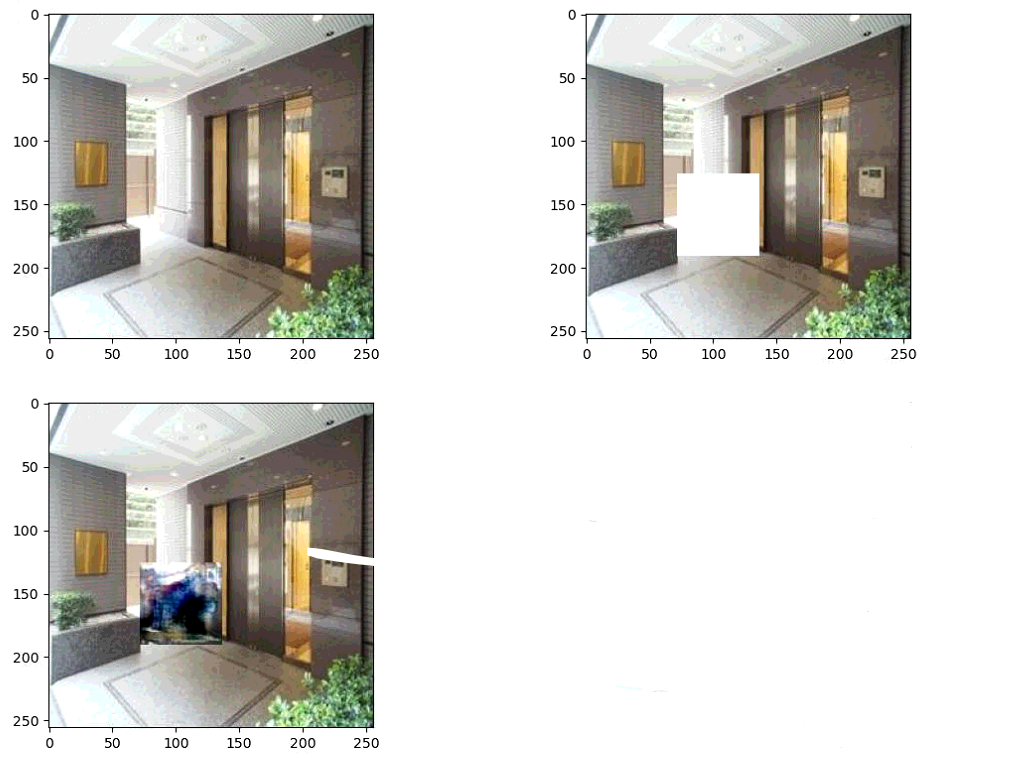
\includegraphics[scale=0.5]{figures/chapter5/testUnified.PNG}
    \caption{Unified Model Inpainting Example !!Duzeltilecek}
    \label{fig:unifiedexample}
\end{figure}

\newpage
\section{Test Results}

Yazilacak.